%\ctparttext{\color{black}\begin{center}
%		Esta es una descripción de la parte de informática.
%\end{center}}

%\part{Parte de informática}
\chapter{Tablas}

En esta sección se presentarán algunos conceptos y herramientas básicas que nos resultarán útiles a lo largo de los siguientes capítulos.

\section{Caso 1}

\subsection{Algoritmos}

\begin{table}[H]
\centering
\caption{Caso 1 - Resultados de ejecución de algoritmos.}
\label{tab:c1_alg}
\begin{tabular}{ccccc}
\toprule
 Algoritmo & Tiempo (s) & Silhouette & Calinski-Harabasz & Número de clusters \\
\midrule
kmeans & 0.057 & 625.999 & 0.33432 & 5 \\
birch & 0.106 & 336.711 & 0.48426 & 5 \\
spectral & 0.646 & 534.083 & 0.29880 & 5 \\
dbscan & 0.126 & 333.456 & 0.67367 & 2 \\
meanshift & 10.410 & 73.801 & 0.35908 & 32 \\
\bottomrule
\end{tabular}
\end{table}

\subsection{Parametros dbscan}

\begin{table}[H]
\centering
\caption{Caso 1 - Cambio de parámetros DBSCAN}
\label{tab:c1_dbscan}
\begin{tabular}{ccccccc}
\toprule
Algoritmo & eps & min samples & Tiempo(s) & Silhouette & Calinski-Harabasz & n clusters \\
\midrule
dbscan & 0.126 & 15.000 & 0.129 & 314.352 & 0.67749 & 2 \\
dbscan & 0.126 & 20.000 & 0.125 & 333.456 & 0.67367 & 2 \\
dbscan & 0.126 & 25.000 & 0.121 & 354.162 & 0.66902 & 2 \\
dbscan & 0.126 & 30.000 & 0.125 & 368.859 & 0.66260 & 2 \\
dbscan & 0.126 & 35.000 & 0.128 & 376.451 & 0.65698 & 2 \\
dbscan & 0.130 & 15.000 & 0.127 & 323.611 & 0.68333 & 2 \\
dbscan & 0.130 & 20.000 & 0.121 & 338.608 & 0.67757 & 2 \\
dbscan & 0.130 & 25.000 & 0.130 & 354.371 & 0.67411 & 2 \\
dbscan & 0.130 & 30.000 & 0.123 & 359.105 & 0.67258 & 2 \\
dbscan & 0.130 & 35.000 & 0.124 & 366.292 & 0.66568 & 2 \\
dbscan & 0.150 & 15.000 & 0.135 & 288.264 & 0.70224 & 2 \\
dbscan & 0.150 & 20.000 & 0.134 & 304.901 & 0.69936 & 2 \\
dbscan & 0.150 & 25.000 & 0.132 & 311.673 & 0.69243 & 2 \\
dbscan & 0.150 & 30.000 & 0.132 & 319.038 & 0.68550 & 2 \\
dbscan & 0.150 & 35.000 & 0.132 & 321.172 & 0.68152 & 2 \\
dbscan & 0.170 & 15.000 & 0.143 & 281.696 & 0.71489 & 2 \\
dbscan & 0.170 & 20.000 & 0.137 & 279.062 & 0.70922 & 2 \\
dbscan & 0.170 & 25.000 & 0.139 & 286.660 & 0.70839 & 2 \\
dbscan & 0.170 & 30.000 & 0.138 & 295.586 & 0.70562 & 2 \\
dbscan & 0.170 & 35.000 & 0.145 & 294.783 & 0.70345 & 2 \\
dbscan & 0.200 & 15.000 & 0.145 & 231.341 & 0.73756 & 2 \\
dbscan & 0.200 & 20.000 & 0.143 & 228.641 & 0.72741 & 2 \\
dbscan & 0.200 & 25.000 & 0.144 & 239.060 & 0.72724 & 2 \\
dbscan & 0.200 & 30.000 & 0.141 & 248.309 & 0.72676 & 2 \\
dbscan & 0.200 & 35.000 & 0.141 & 269.916 & 0.72272 & 2 \\
\bottomrule
\end{tabular}
\end{table}



\subsection{Parametros birch}


\begin{table}[H]
\centering
\caption{Caso 1 - Cambio de parámetros Birch}
\label{tab:c1_birch}
\begin{tabular}{ccccccc}
\toprule
Algoritmo & Branch fact & Threshold & Tiempo(s) & Silhouette & Calinski-Harabasz & n clusters \\
\midrule
birch & 15.000 & 0.100 & 0.087 & 336.711 & 0.48426 & 5 \\
birch & 15.000 & 0.150 & 0.065 & 192.073 & 0.58865 & 5 \\
birch & 15.000 & 0.200 & 0.060 & 206.873 & 0.60273 & 5 \\
birch & 15.000 & 0.250 & 0.062 & 206.873 & 0.60273 & 1 \\
birch & 15.000 & 0.300 & 0.049 & 206.873 & 0.60273 & 1 \\
birch & 20.000 & 0.100 & 0.147 & 173.266 & 0.58162 & 5 \\
birch & 20.000 & 0.150 & 0.077 & 180.842 & 0.58567 & 5 \\
birch & 20.000 & 0.200 & 0.046 & 206.873 & 0.60273 & 5 \\
birch & 20.000 & 0.250 & 0.053 & 206.873 & 0.60273 & 1 \\
birch & 20.000 & 0.300 & 0.052 & 206.873 & 0.60273 & 1 \\
birch & 25.000 & 0.100 & 0.153 & 312.603 & 0.49236 & 5 \\
birch & 25.000 & 0.150 & 0.064 & 184.304 & 0.57974 & 5 \\
birch & 25.000 & 0.200 & 0.045 & 206.873 & 0.60273 & 5 \\
birch & 25.000 & 0.250 & 0.051 & 206.873 & 0.60273 & 1 \\
birch & 25.000 & 0.300 & 0.043 & 206.873 & 0.60273 & 1 \\
birch & 30.000 & 0.100 & 0.136 & 292.036 & 0.52240 & 5 \\
birch & 30.000 & 0.150 & 0.059 & 184.304 & 0.57974 & 5 \\
birch & 30.000 & 0.200 & 0.066 & 206.873 & 0.60273 & 5 \\
birch & 30.000 & 0.250 & 0.057 & 206.873 & 0.60273 & 1 \\
birch & 30.000 & 0.300 & 0.074 & 206.873 & 0.60273 & 1 \\
birch & 35.000 & 0.100 & 0.129 & 355.783 & 0.42852 & 5 \\
birch & 35.000 & 0.150 & 0.058 & 184.304 & 0.57974 & 5 \\
birch & 35.000 & 0.200 & 0.061 & 206.873 & 0.60273 & 5 \\
birch & 35.000 & 0.250 & 0.061 & 206.873 & 0.60273 & 1 \\
birch & 35.000 & 0.300 & 0.054 & 206.873 & 0.60273 & 1 \\
\bottomrule
\end{tabular}
\end{table}

\begin{figure}
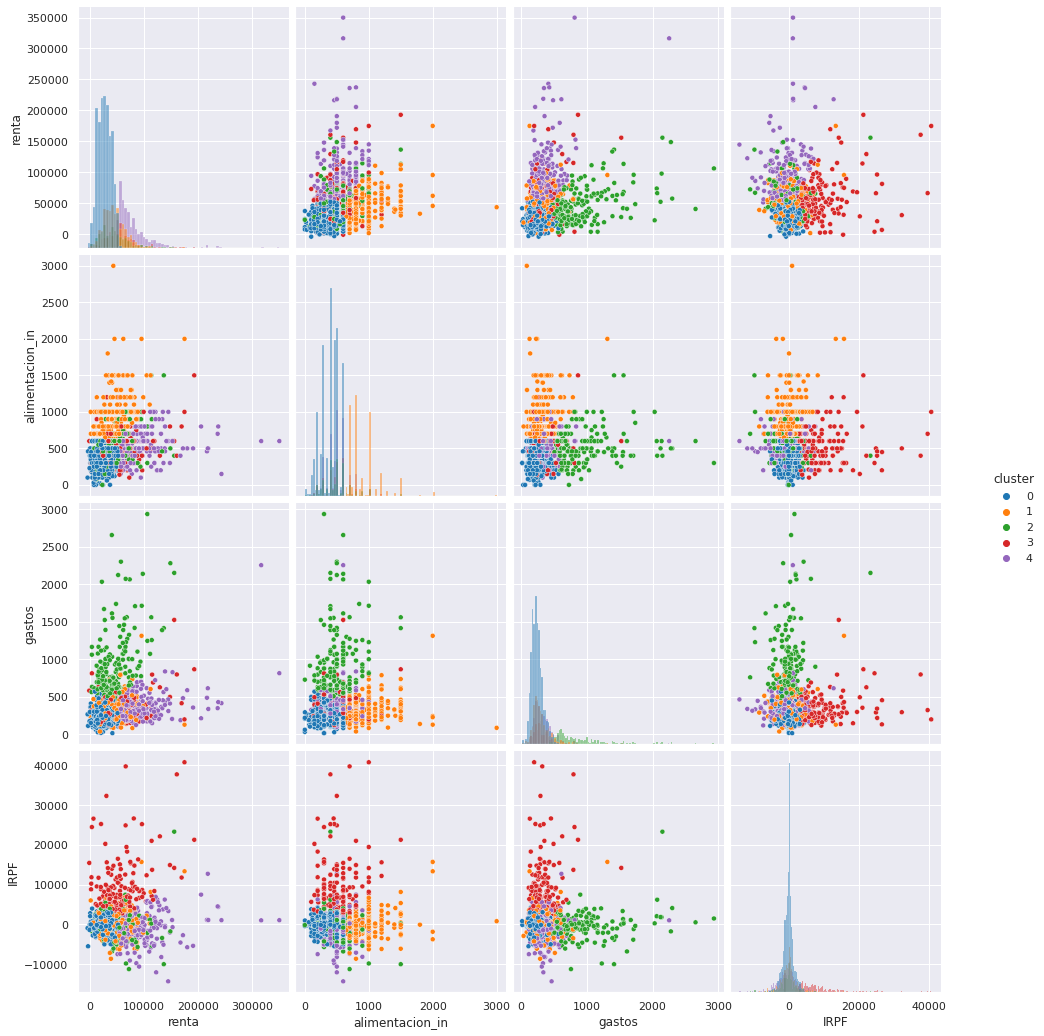
\includegraphics[scale=0.45]{caso1/kmeans/scatter.png}
\end{figure}